\chapter{Introduction to Optical Fiber Communication}



\section{Section 1: Basics of Optical Communication [10M] [Priority: High]}

\subsection{1. General vs. Fiber Optic Communication Systems}
A communication system transmits information from a source to a destination. In an optical communication system, light is used as the information carrier, and the transmission medium is an optical fiber cable.

\subsubsection{A. General Communication System Block Diagram}
A standard communication system consists of three main elements: Transmitter, Channel, and Receiver.

\begin{figure}[H]
\centering
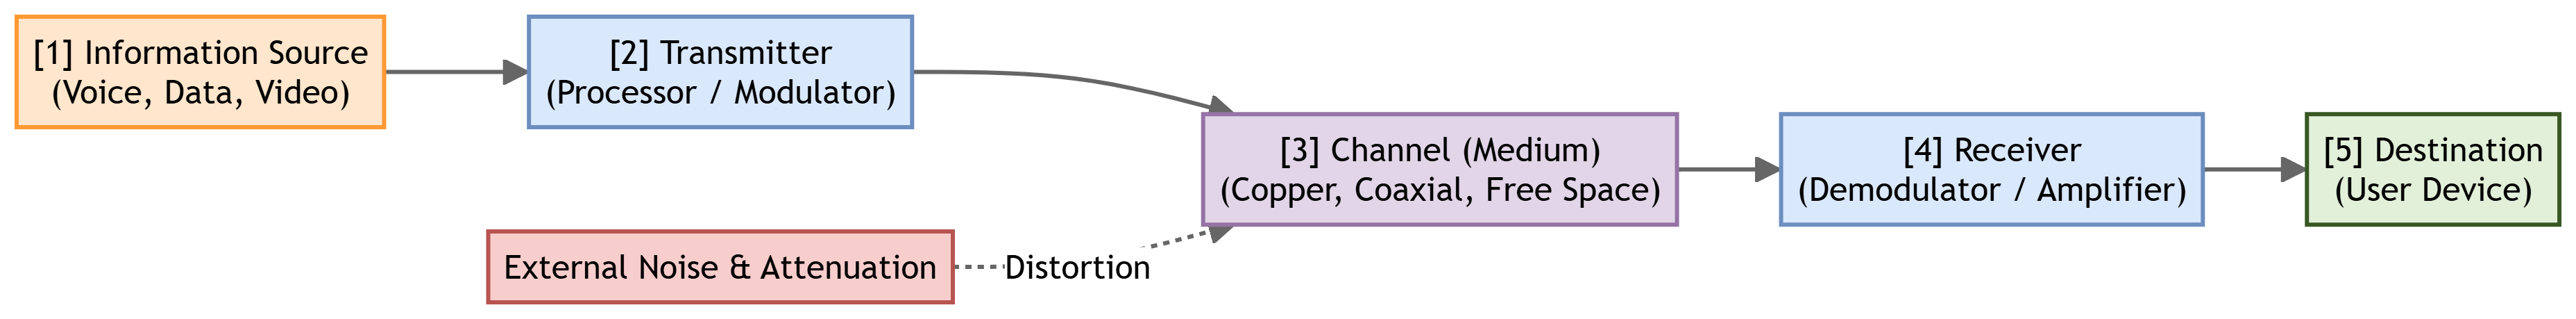
\includegraphics[width=0.75\textwidth,height=0.32\textheight,keepaspectratio]{../Images/chapter_01/general_comm_block.png}
\caption{General Communication System Block Diagram}
\end{figure}

\begin{enumerate}
  \item \textbf{Information Source:} Generates the input message signal (analog voice, digital data, video).
  \item \textbf{Transmitter:} Processes and modulates the source signal onto a suitable carrier wave (RF, microwave) for transmission.
  \item \textbf{Channel (Medium):} The physical path over which the modulated signal propagates (free space, copper wire, coaxial cable). Noise and attenuation degrade the signal here.
  \item \textbf{Receiver:} Demodulates and amplifies the received signal, converting it back to the original message format.
  \item \textbf{Destination:} The final recipient of the transmitted message.
\end{enumerate}

\subsubsection{B. Fiber Optic Communication System Block Diagram}
An optical fiber communication system adapts the general framework to use light signals and optical fibers.

\begin{figure}[H]
\centering
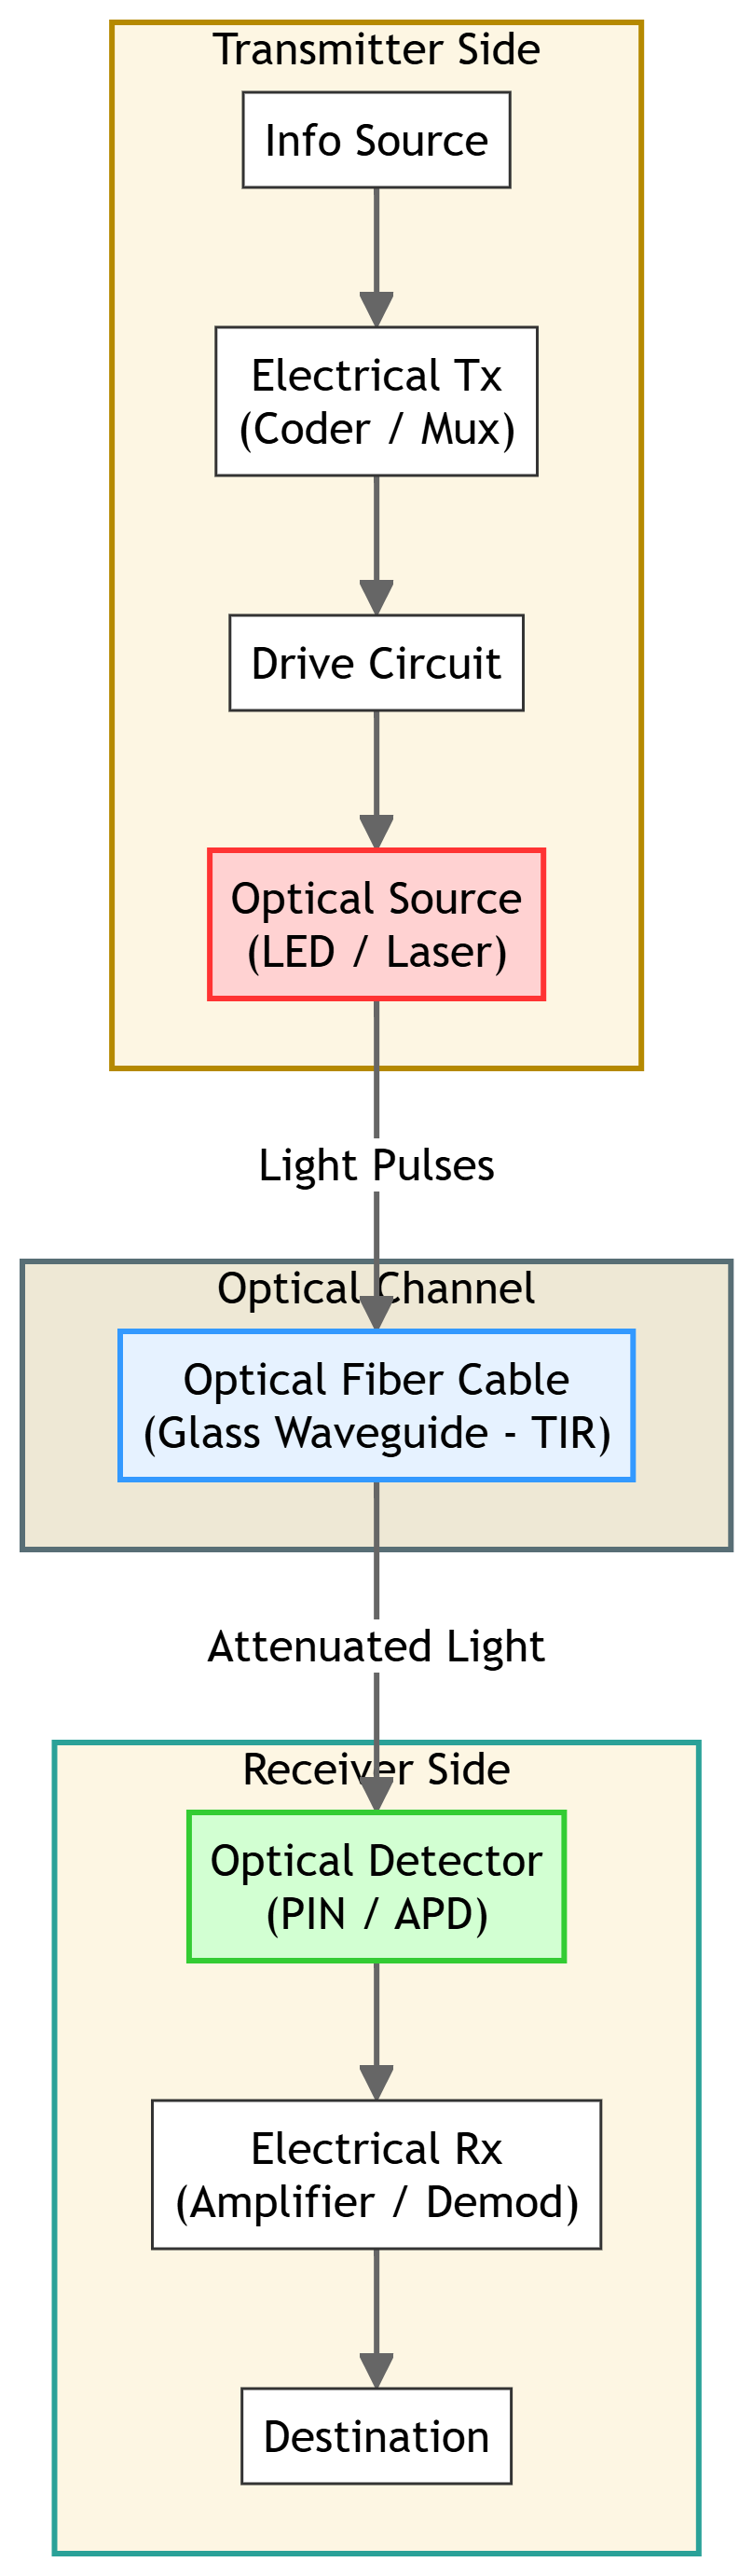
\includegraphics[width=0.75\textwidth,height=0.32\textheight,keepaspectratio]{../Images/chapter_01/fiber_comm_block.png}
\caption{Fiber Optic Communication System Block Diagram}
\end{figure}

\begin{enumerate}
  \item \textbf{Information Source \& Electrical Transmitter:} Converts non-electrical messages (like voice) into electrical signals and processes them (coding, multiplexing).
  \item \textbf{Drive Circuit:} Modulates the electrical signal into a drive current suitable for operating the optical source.
  \item \textbf{Optical Source:} Converts electrical signal variations into light pulses.
\end{enumerate}
    \textit{   }LED (Light Emitting Diode):* Used for low-speed, short-distance transmission.
    \textit{   }Laser Diode:* Used for high-speed, long-distance transmission.
\begin{enumerate}
  \item \textbf{Optical Fiber Cable (Channel):} A cylindrical glass/plastic waveguide that guides light pulses via \textbf{Total Internal Reflection (TIR)}.
  \item \textbf{Optical Detector (Photodetector):} Converts the received light pulses back into electrical current.
\end{enumerate}
    \textit{   }PIN Photodiode:* Simple, low noise, no internal gain.
    \textit{   }APD (Avalanche Photodiode):* High sensitivity, high response speed, possesses internal multiplication gain.
\begin{enumerate}
  \item \textbf{Electrical Receiver (Amplifier/Demodulator):} Amplifies the weak photodetector current, filters out noise, and reconstructs the original signal.
  \item \textbf{Destination:} The end-user device or computer system.
\end{enumerate}


\subsection{2. Advantages \& Disadvantages of Optical Fiber Communication}

\subsubsection{A. Advantages}
\begin{itemize}
  \item   \textbf{Enormous Bandwidth:} Light frequencies are in the terahertz range ($10^{14}\ \text{Hz}$), providing a transmission bandwidth-distance product thousands of times greater than copper cables or microwave links.
  \item   \textbf{Low Attenuation (Transmission Loss):} Modern silica glass fibers have losses as low as $0.2\ \text{dB/km}$ at $\lambda = 1550\ \text{nm}$, allowing signal transmission over $100\ \text{km}$ without repeaters.
  \item   \textbf{Immunity to Electromagnetic Interference (EMI):} Being made of dielectric materials (glass/plastic), fibers are completely unaffected by external magnetic fields, lightning strikes, high-voltage lines, or radio frequency signals.
  \item   \textbf{Small Size and Lightweight:} An optical fiber has a core/cladding diameter of about $125\ \mu\text{m}$, making cables much thinner and lighter than copper bundles.
  \item   \textbf{High Security \& No Crosstalk:} Light is confined entirely within the fiber core. There is no electromagnetic radiation escaping the cable, making unauthorized tapping virtually impossible and eliminating crosstalk between adjacent fibers.
  \item   \textbf{Electrical Isolation:} Since fibers are non-conductive, there is no risk of electrical shocks, short circuits, or ground loops, making them safe for hazardous environments (chemical plants, oil refineries).
\end{itemize}

\subsubsection{B. Disadvantages}
\begin{itemize}
  \item   \textbf{High Initial Installation Cost:} The cost of specialized optical transmitters, receivers, and deployment equipment is higher than copper equivalents.
  \item   \textbf{Fragility and Splicing Difficulty:} Glass fibers are fragile and susceptible to damage under bending stress. Splicing (joining) two fibers requires expensive fusion splicing tools and highly skilled technicians.
  \item   \textbf{Specialized Components:} Optical connectors, splitters, and amplifiers are complex to design and align.
  \item   \textbf{Cannot Carry Electrical Power:} Unlike copper wires, optical fibers cannot transmit electrical power directly to remote equipment (e.g., telephone sets, sensors).
\end{itemize}


\section{Section 2: Ray Optics \& Light Propagation Principles [15M] [Priority: High]}

Light propagation in large-core fibers ($d \gg \lambda$) is modeled using \textbf{Geometric (Ray) Optics}, assuming light travels in straight lines (rays) and changes direction at interfaces between different media.

\subsection{1. Refraction, Snell's Law, Critical Angle, and Total Internal Reflection (TIR)}

\begin{itemize}
  \item   \textbf{Refraction:} The bending of a light ray as it passes from one transparent medium with refractive index $n_1$ to another with refractive index $n_2$, caused by the change in the speed of light.
  \item   \textbf{Snell's Law:} Governs refraction at the interface of two media:
\end{itemize}
    \[ n_1 \sin(\theta_1) = n_2 \sin(\theta_2) \]
    where $\theta_1$ is the angle of incidence and $\theta_2$ is the angle of refraction.

\begin{itemize}
  \item   \textbf{Critical Angle ($\theta_c$):} When light travels from a denser medium ($n_1$) to a rarer medium ($n_2$, where $n_1 > n_2$), the refracted ray bends away from the normal. As the angle of incidence ($\theta_1$) increases, the angle of refraction ($\theta_2$) reaches $90^\circ$ (propagating along the interface). The angle of incidence that causes $\theta_2 = 90^\circ$ is the \textbf{Critical Angle ($\theta_c$)}:
\end{itemize}
    \[ n_1 \sin(\theta_c) = n_2 \sin(90^\circ) \implies \theta_c = \sin^{-1}\left(\frac{n_2}{n_1}\right) \]

\begin{itemize}
  \item   \textbf{Total Internal Reflection (TIR):} The phenomenon where a light ray traveling in a denser medium hits the interface with a rarer medium and is entirely reflected back into the denser medium.
\end{itemize}
    \textit{   }Conditions for TIR:*
\begin{enumerate}
  \item The light ray must travel from a medium of higher refractive index ($n_1$) to a medium of lower refractive index ($n_2$) ($n_1 > n_2$).
  \item The angle of incidence at the interface must exceed the critical angle ($\theta_i > \theta_c$).
\end{enumerate}


\subsection{2. Acceptance Angle \& Numerical Aperture (NA) Derivation}

The \textbf{Acceptance Angle ($\theta_a$)} is the maximum angle of incidence at the air-core interface for which the light ray will be totally internally reflected at the core-cladding interface and thus propagate along the fiber. The \textbf{Numerical Aperture (NA)} represents the light-gathering capacity of the fiber.

\begin{figure}[H]
\centering
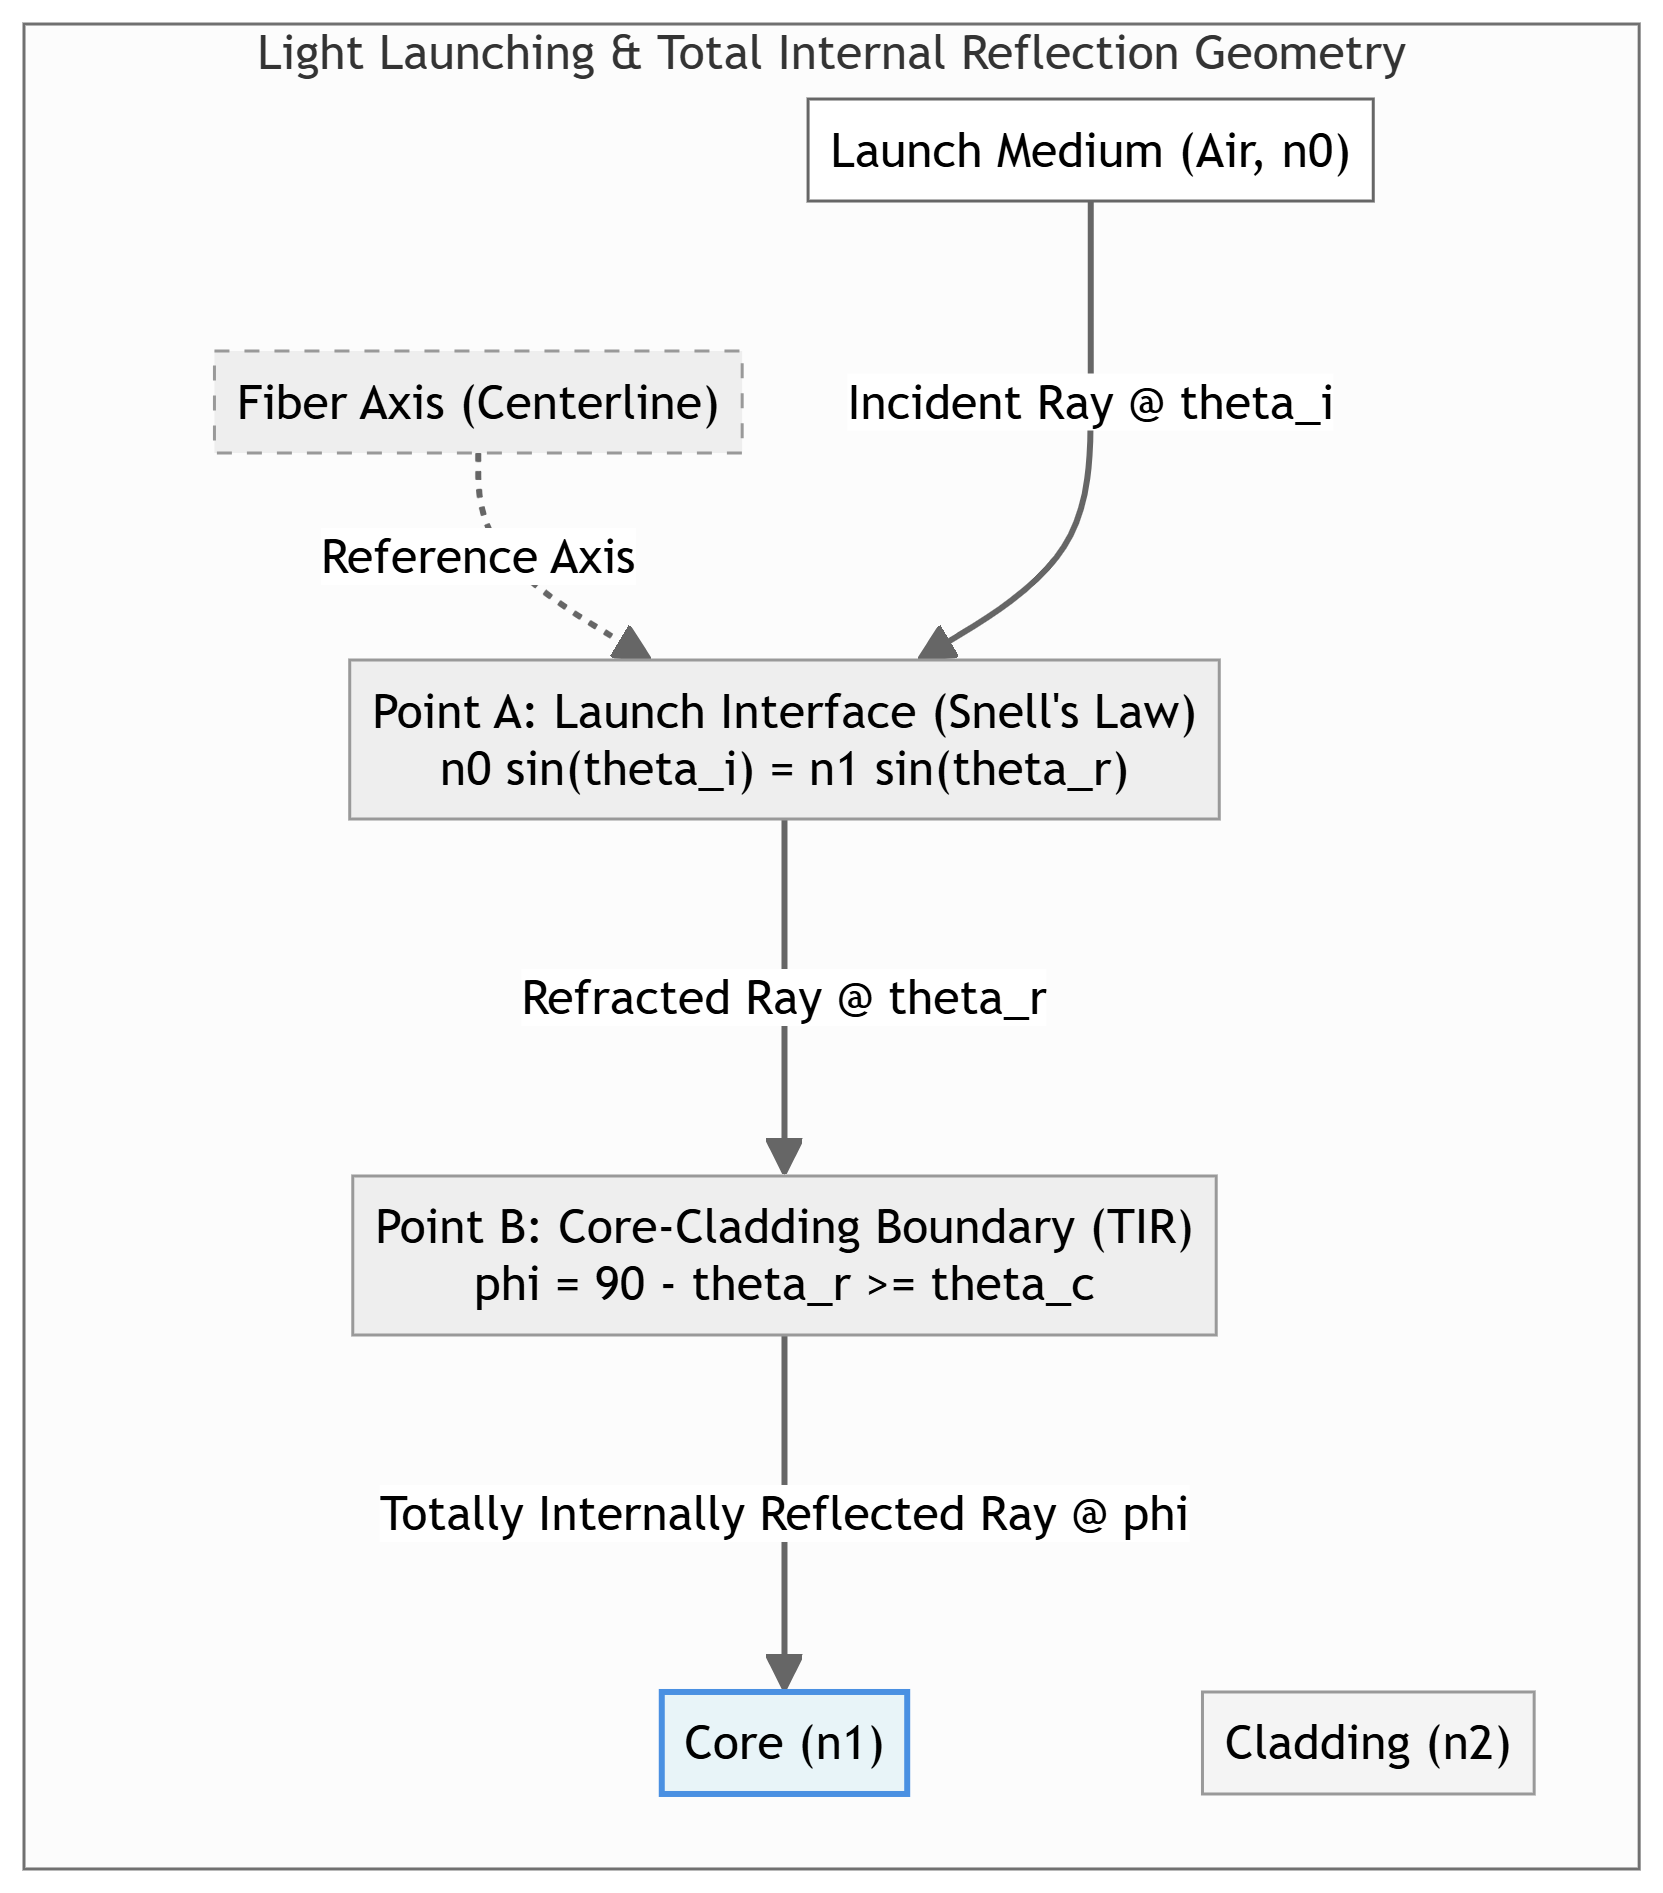
\includegraphics[width=0.75\textwidth,height=0.32\textheight,keepaspectratio]{../Images/chapter_01/ray_propagation.png}
\caption{Ray Propagation \& Acceptance Angle}
\end{figure}

\subsubsection{Step-by-Step Derivation:}
\begin{enumerate}
  \item Let $n_0$ be the refractive index of the launching medium (usually air, $n_0 = 1$), $n_1$ be the core refractive index, and $n_2$ be the cladding refractive index ($n_1 > n_2$).
  \item Let a light ray enter the fiber core from the launching medium at an angle of incidence $\theta_i$ with the fiber axis. Let $\theta_r$ be the angle of refraction inside the core.
  \item By \textbf{Snell's Law} at the air-core interface (Point A):
\end{enumerate}
    \[ n_0 \sin(\theta_i) = n_1 \sin(\theta_r) \quad \text{--- (Eq 1.1)} \]
\begin{enumerate}
  \item The refracted ray travels through the core and strikes the core-cladding interface (Point B) at an angle of incidence $\phi$. From the geometry of the right-angled triangle ABC:
\end{enumerate}
    \[ \phi = 90^\circ - \theta_r \quad \text{--- (Eq 1.2)} \]
\begin{enumerate}
  \item For the ray to undergo Total Internal Reflection (TIR) at Point B, we must have:
\end{enumerate}
    \[ \phi \ge \theta_c \implies \sin(\phi) \ge \sin(\theta_c) \]
\begin{enumerate}
  \item Since $\sin(\theta_c) = \frac{n_2}{n_1}$, this condition becomes:
\end{enumerate}
    \[ \sin(\phi) \ge \frac{n_2}{n_1} \quad \text{--- (Eq 1.3)} \]
\begin{enumerate}
  \item Using Eq 1.2, we rewrite $\sin(\phi)$ as:
\end{enumerate}
    \[ \sin(\phi) = \sin(90^\circ - \theta_r) = \cos(\theta_r) \]
\begin{enumerate}
  \item Substituting this into Eq 1.3:
\end{enumerate}
    \[ \cos(\theta_r) \ge \frac{n_2}{n_1} \]
\begin{enumerate}
  \item Using the trigonometric identity $\sin(\theta_r) = \sqrt{1 - \cos^2(\theta_r)}$:
\end{enumerate}
    \[ \sin(\theta_r) \le \sqrt{1 - \left(\frac{n_2}{n_1}\right)^2} = \sqrt{\frac{n_1^2 - n_2^2}{n_1^2}} = \frac{\sqrt{n_1^2 - n_2^2}}{n_1} \]
\begin{enumerate}
  \item Substitute this inequality back into Snell's Law (Eq 1.1):
\end{enumerate}
    \[ n_0 \sin(\theta_i) \le n_1 \left( \frac{\sqrt{n_1^2 - n_2^2}}{n_1} \right) = \sqrt{n_1^2 - n_2^2} \]
\begin{enumerate}
  \item The maximum angle of incidence $\theta_i = \theta_a$ (Acceptance Angle) occurs at the limit:
\end{enumerate}
    \[ \sin(\theta_a) = \frac{\sqrt{n_1^2 - n_2^2}}{n_0} \]
\begin{enumerate}
  \item For air launching ($n_0 = 1$), the \textbf{Acceptance Angle ($\theta_a$)} is:
\end{enumerate}
    \[ \theta_a = \sin^{-1}\left(\sqrt{n_1^2 - n_2^2}\right) \]
\begin{enumerate}
  \item The \textbf{Numerical Aperture (NA)} is defined as the sine of the acceptance angle in air:
\end{enumerate}
    \[ \text{NA} = \sin(\theta_a) = \sqrt{n_1^2 - n_2^2} \]
\begin{enumerate}
  \item Using the \textbf{Relative Refractive Index Difference ($\Delta$)}:
\end{enumerate}
    \[ \Delta = \frac{n_1^2 - n_2^2}{2 n_1^2} \approx \frac{n_1 - n_2}{n_1} \]
    We can rewrite the expression as:
    \[ n_1^2 - n_2^2 = 2 n_1^2 \Delta \implies \text{NA} = n_1 \sqrt{2 \Delta} \]


\subsection{3. Meridional vs. Skew Rays}
Light rays propagating along an optical fiber are classified based on their path and intersection with the fiber's central axis.

\begin{table}[H]
\centering
\begin{tabular}{|p{\dimexpr 0.2\textwidth - 2\tabcolsep - 1.5\arrayrulewidth\relax}|p{\dimexpr 0.4\textwidth - 2\tabcolsep - 1.5\arrayrulewidth\relax}|p{\dimexpr 0.4\textwidth - 2\tabcolsep - 1.5\arrayrulewidth\relax}|}
\hline
Feature / Criteria & Meridional Rays & Skew Rays \\
\hline
\textbf{Path Definition} & Pass through the fiber's longitudinal axis. & Do not pass through the fiber's longitudinal axis. \\
\hline
\textbf{Propagation Geometry} & Confined to a single plane containing the axis (meridional plane). & Follow a helical or spiral path around the axis. \\
\hline
\textbf{Mathematical Analysis} & Simple; modeled using 2D geometry and ray tracing. & Complex; requires 3D cylindrical geometry. \\
\hline
\textbf{Acceptance Condition} & Determined by the standard NA equation: $\sin(\theta_a) = \text{NA}$. & Can be accepted at larger launch angles than meridional rays. \\
\hline
\textbf{Total Internal Reflection} & Occurs at a flat cylindrical surface point. & Occurs along a helical trajectory path at the core boundary. \\
\hline
\end{tabular}
\end{table}


\section{Section 3: Electromagnetic Model \& Vector Nature of Light [5M] [Priority: Medium]}

When the core diameter ($d$) of the fiber is comparable to the wavelength of the light ($\lambda$), geometric optics fails. In this regime, light must be modeled as electromagnetic waves using Maxwell's equations.

\subsection{1. Ray Model vs. Wave Model}

\begin{table}[H]
\centering
\begin{tabular}{|p{\dimexpr 0.2\textwidth - 2\tabcolsep - 1.5\arrayrulewidth\relax}|p{\dimexpr 0.4\textwidth - 2\tabcolsep - 1.5\arrayrulewidth\relax}|p{\dimexpr 0.4\textwidth - 2\tabcolsep - 1.5\arrayrulewidth\relax}|}
\hline
Feature / Criteria & Ray Model (Geometric Optics) & Wave Model (Waveguide Theory) \\
\hline
\textbf{Light Representation} & Discrete light rays traveling in straight lines. & Continuous electromagnetic waves (E \& H fields). \\
\hline
\textbf{Wavelength Assumption} & Assumes wavelength is negligible ($\lambda \to 0$). & Accounts for finite wavelength ($\lambda$). \\
\hline
\textbf{Fiber Compatibility} & Valid only for multimode fibers ($d \gg \lambda$). & Mandatory for single-mode fibers ($d \approx \lambda$). \\
\hline
\textbf{Target Phenomena} & Describes refraction, reflection, critical angle, and NA. & Explains diffraction, interference, modal cutoff, and dispersion. \\
\hline
\textbf{Resulting Concept} & Light paths (continuous geometric angles). & Discrete electromagnetic modes (guided wave patterns). \\
\hline
\end{tabular}
\end{table}


\subsection{2. Vector Nature of Light \& cylindrical Dielectric Rod}
Light waves consist of oscillating electric ($\vec{E}$) and magnetic ($\vec{H}$) fields, which are vectors perpendicular to each other and to the direction of propagation.

\begin{itemize}
  \item   \textbf{Maxwell's Equations:} Light propagation in a cylindrical dielectric rod (representing the fiber core) is modeled by solving the electromagnetic wave equations in cylindrical coordinates $(r, \phi, z)$:
\end{itemize}
    \[ \nabla^2 \vec{E} - n^2 \mu_0 \epsilon_0 \frac{\partial^2 \vec{E}}{\partial t^2} = 0 \]
\begin{itemize}
  \item   \textbf{Modes of Propagation:} Because of the vector boundary conditions at the cylindrical core-cladding interface, the electromagnetic waves cannot propagate as simple transverse electromagnetic (TEM) waves. Instead, they form discrete modes:
\end{itemize}
\begin{enumerate}
  \item \textbf{Transverse Electric (TE) Modes:} No electric field component in the direction of propagation ($E_z = 0$).
  \item \textbf{Transverse Magnetic (TM) Modes:} No magnetic field component in the direction of propagation ($H_z = 0$).
  \item \textbf{Hybrid Modes (HE and EH):} Both electric and magnetic fields have non-zero components in the direction of propagation ($E_z \neq 0, H_z \neq 0$). These arise because of skew rays and the cylindrical boundary curvature.
\end{enumerate}


\section{Section 4: Practice Problems [10M] [Priority: High]}

\subsection{Problem 1.1: Critical Angle Calculation}
\textbf{Given:}
\begin{itemize}
  \item   Core refractive index ($n_1$) = \textbf{1.82}
  \item   Cladding refractive index ($n_2$) = \textbf{1.73}
\end{itemize}

\textbf{Formula:}
\[ \theta_c = \sin^{-1}\left(\frac{n_2}{n_1}\right) \]

\textbf{Substitution \& Calculation:}
\[ \theta_c = \sin^{-1}\left(\frac{1.73}{1.82}\right) \]
\[ \theta_c = \sin^{-1}(0.95055) \]
\[ \theta_c \approx 71.91^\circ \]

\textbf{Final Answer:}
The critical angle at the core-cladding interface is \textbf{$71.91^\circ$}.


\subsection{Problem 1.2: Numerical Aperture \& Index Tuning}
\textbf{Given:}
\begin{itemize}
  \item   Core refractive index ($n_1$) = \textbf{1.48}
  \item   Cladding refractive index ($n_2$) = \textbf{1.46}
  \item   Target NA = \textbf{0.23}
\end{itemize}

\textbf{Formulas:}
\begin{enumerate}
  \item $\text{NA} = \sqrt{n_1^2 - n_2^2}$
  \item $n_2' = \sqrt{n_1^2 - (\text{NA}')^2}$
\end{enumerate}

\textbf{Step 1: Calculate the initial NA:}
\[ \text{NA} = \sqrt{(1.48)^2 - (1.46)^2} \]
\[ \text{NA} = \sqrt{2.1904 - 2.1316} = \sqrt{0.0588} \]
\[ \text{NA} \approx 0.242 \]

\textbf{Step 2: Calculate the new cladding index ($n_2'$) for target $\text{NA} = 0.23$:}
\[ n_2' = \sqrt{(1.48)^2 - (0.23)^2} \]
\[ n_2' = \sqrt{2.1904 - 0.0529} = \sqrt{2.1375} \]
\[ n_2' \approx 1.462 \]

\textbf{Final Answer:}
\begin{itemize}
  \item   The initial Numerical Aperture is \textbf{0.242}.
  \item   The new cladding refractive index ($n_2'$) required to change the NA to $0.23$ is \textbf{1.462}.
\end{itemize}


\subsection{Problem 1.3: Acceptance Angle in Air}
\textbf{Given:}
\begin{itemize}
  \item   Core refractive index ($n_1$) = \textbf{1.50}
  \item   Cladding refractive index ($n_2$) = \textbf{1.47}
  \item   Launch medium = Air ($n_0 = 1$)
\end{itemize}

\textbf{Formulas:}
\begin{enumerate}
  \item Critical Angle: $\theta_c = \sin^{-1}\left(\frac{n_2}{n_1}\right)$
  \item Numerical Aperture: $\text{NA} = \sqrt{n_1^2 - n_2^2}$
  \item Acceptance Angle: $\theta_a = \sin^{-1}(\text{NA})$
\end{enumerate}

\textbf{Substitution \& Calculation:}
\begin{enumerate}
  \item \textbf{Critical Angle ($\theta_c$):}
\end{enumerate}
    \[ \theta_c = \sin^{-1}\left(\frac{1.47}{1.50}\right) = \sin^{-1}(0.98) \]
    \[ \theta_c \approx 78.52^\circ \]
\begin{enumerate}
  \item \textbf{Numerical Aperture (NA):}
\end{enumerate}
    \[ \text{NA} = \sqrt{(1.50)^2 - (1.47)^2} = \sqrt{2.25 - 2.1609} = \sqrt{0.0891} \]
    \[ \text{NA} \approx 0.2985 \]
\begin{enumerate}
  \item \textbf{Acceptance Angle ($\theta_a$):}
\end{enumerate}
    \[ \theta_a = \sin^{-1}(0.2985) \]
    \[ \theta_a \approx 17.37^\circ \]

\textbf{Final Answer:}
\begin{itemize}
  \item   The critical angle is \textbf{$78.52^\circ$}.
  \item   The Numerical Aperture is \textbf{0.2985}.
  \item   The acceptance angle in air is \textbf{$17.37^\circ$}.
\end{itemize}
